\begin{center}
    \begin{figure}[H]
        \centering

        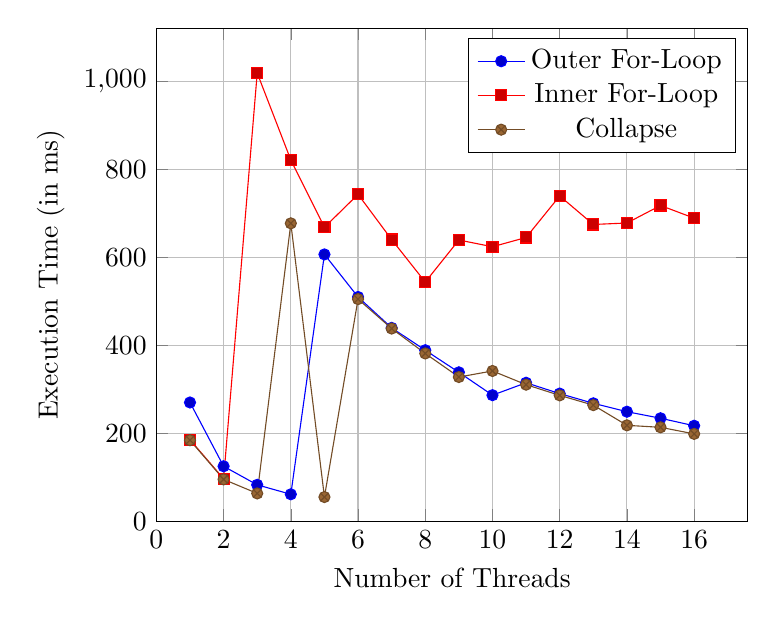
\begin{tikzpicture}
            \begin{axis}[
                title={},
                width=0.75\textwidth,
                xlabel={Number of Threads},
                ylabel={Execution Time (in ms)},
                xmin=0,
                ymin=0,
                grid=major
            ]
                \addplot coordinates {
                    (1,270.144)(2,125.102)(3,82.8802)(4,61.4252)(5,606.726)(6,509.935)(7,439.723)(8,388.928)(9,338.68)(10,286.706)(11,314.933)(12,290.336)(13,268.227)(14,249.136)(15,234.278)(16,217.202)
                };
                \addlegendentry{Outer For-Loop}

                \addplot coordinates {
                    (1,185.42)(2,96.6801)(3,1019.01)(4,821.332)(5,668.312)(6,743.242)(7,640.431)(8,543.896)(9,639.406)(10,624.191)(11,645.23)(12,739.567)(13,674.792)(14,678.1)(15,717.971)(16,689.155)
                };
                \addlegendentry{Inner For-Loop}       

                \addplot coordinates {
                    (1,184.356)(2,95.3219)(3,63.3876)(4,677.361)(5,55.1428)(6,505.167)(7,438.152)(8,381.56)(9,327.991)(10,341.76)(11,310.625)(12,286.291)(13,264.068)(14,218.169)(15,213.658)(16,198.713)
                };
                \addlegendentry{Collapse}
            \end{axis}
        \end{tikzpicture}
        \caption{HSV Performance Tests dice\_large.png}
    \end{figure}
\end{center}